\chapter{Desenvolvimento}

\indent No capítulo de desenvolvimento serão apresentadas informações referentes à base de dados, suas características e o processo de preparação da mesma para a aplicação do algoritmo K-means. Também serão apresentados detalhes sobre a implementação do algoritmo, experimentos realizados e os resultados obtidos.

  \section{Base de Dados}

\indent A base de dados KDDcup99 \cite{kdd99} é um dos conjuntos de dados mais utilizados para avaliação de sistemas de detecção de anomalias e detecção de intrusões. A KDD99 foi elaborada à partir dos dados do tráfego gerado artificialmente no DARPA 98, criado pelo Laboratório Lincoln do Instituto Tecnológico de Massachusetts para avaliação de sistemas de detecção de intrusão.

\indent A base contém aproximadamente quatro milhões e novecentos mil vetores de conexões, que são compostos por 42 atributos referentes aos recursos utilizados em cada conexão. Cada vetor de conexão possui uma rotulagem, que pode ser normal ou de algum determinado ataque. Apesar da incerteza no que se refere à efetividade do tráfego gerado artificialmente, este conjunto de dados é utilizado em grande escala na literatura, além disso, a tarefa de clusterização não sofre influência em relação à origem dos dados.

\begin{table}[h]
\centering
\caption{Atributos dos vetores de conexão.}
\vspace{0.5cm}
\begin{tabular}{|r|l|r|l|}
\hline
\textbf{Nº} & \textbf{Nome do Atributo} & \textbf{Nº} & \textbf{Nome do Atributo} \\
\hline                               
1 & Duration 	  & 22 & Count \\
\hline
2 & Protocol\_type & 23 & Srv\_count \\
\hline
3 & Service    	  & 24 & Serror\_rate \\
\hline
4 & Flag          & 25 & Srv\_serror\_rate \\
\hline
5 & Src\_bytes    & 26 & Error\_rate \\
\hline
6 & Dst\_bytes	  & 27 & Srv\_rerror\_rate \\
\hline
7 & Land	  & 28 & Same\_srv\_rate \\
\hline
8 & Wrong\_fragment & 29 & Diff\_srv\_rate \\
\hline
9 & Urgent 	  & 30 & Srv\_diff\_host\_rate \\
\hline
10 & Hot 	  & 31 & Dst\_host\_count \\
\hline
11 & Num\_failed\_logins & 32 & Dst\_host\_srv\_count \\
\hline
12 & Logged\_in   & 33 & Dst\_host\_same\_srv\_count \\
\hline
13 & Num\_compromised & 34 & Dst\_host\_diff\_srv\_rate\\
\hline
14 & Root\_shell  & 35 & Dst\_host\_same\_src\_port\_rate\\
\hline
15 & Su\_attempted & 36 & Dst\_host\_srv\_diff\_host\_rate\\
\hline
16 & Num\_root    & 37	& Dst\_host\_serror\_rate\\
\hline
17 & Num\_files\_creations & 38 & Dst\_host\_srv\_serror\_rate\\
\hline
18 & Num\_shell   & 39 & Dst\_host\_rerror\_rate\\
\hline
19 & Num\_acess\_files & 40 & Dst\_host\_srv\_rerror\_rate\\
\hline
20 & Num\_outbound\_cmds & 41 & Count\\
\hline
21 & Is\_guest\_login & 42 & Attack\_type\\
\hline
\end{tabular}
\label{tab1}
\end{table}

\begin{table}[h!]
\centering
\caption{Ataques agrupados por tipo.}
\vspace{0.5cm}
\begin{tabular}{|l|l|}
\hline
\textbf{Tipos de Ataques} & \textbf{Ataques contidos na KDD99}\\
\hline
DoS &	Back, land, neptune, pod, smurf, teardrop \\
\hline
R2L &	Ftp\_write, guess\_passwd, imap, multihop, phf,\\ & spy, warezclient, warezmaster \\
\hline
U2R &	Buffer\_overflow, load module Pearl, rootkit\\
\hline
Probe &	Ip\_sweep, n\_map, port\_sweep, satan\\
\hline
\end{tabular}
\label{tab2}
\end{table}

\indent Na tabela~\ref{tab1} são apresentados os atributos que compõem cada vetor de conexão e o seu respectivo significado. Na tabela~\ref{tab2} todos tipos de ataques presentes na base de dados são categorizados de acordo com o seu tipo. Esta classificação é importante devido às características semelhantes entre os ataques de mesma categoria, que na clusterização pode refletir em grupos que contenham um ou mais ataques da mesma categoria.

\indent É possível visualizar a forma em que a base de dados é disponibilizada na tabela~\ref{tab3}. Nota-se que há a presença de valores do tipo literal, inteiro e real. Por isso, para aplicar o algoritmo de agrupamento, se faz necessário realizar uma preparação dos dados. A categorização dos dados é exemplificada na tabela~\ref{tab4}, onde os atributos to tipo literal terão seus valores substituídos por valores correspondentes do tipo inteiro. Dessa forma, o algoritmo pode mensurar o valor dos atributos.

\begin{table}[h]
\centering
\caption{Vetor de conexão pré e pós normalização.}
\vspace{0.5cm}
\begin{tabular}{|l|l|}
\hline
\textbf{Estado} & \textbf{Vetor de conexão}\\
\hline
Inicial	 & 0,tcp,http,SF,274,25212,0,0,0,0,0,1,0,0,0,0,0,0,
	\\ & 0,0,0,0,1,6,0.00,0.00,0.00,0.00,1.00,0.00,0.50,39,
	\\ & 137,1.00,0.00,0.03,0.01,0.00,0.00,0.00,0.00.\\
\hline
Normalizado & 0,0,0,0,0,0.00489,0,0,0,0,0,1,0,0,0,0,0,0,0,0,
	   \\& 0,0,0.001957,0.011742,0,0,0,0,1,0,0.5,0.152941,
	   \\& 0.537255,1,0,0.03,0.01,0,0,0,0.\\
\hline

\end{tabular}
\label{tab3}
\end{table}

\begin{table}[h]
\centering
\caption{Categorização dos protocolos de rede.}
\vspace{0.5cm}
\begin{tabular}{|l|c|}
\hline
\textbf{Protocolo} & \textbf{Valor Categórico}\\
\hline
TCP & 0\\
\hline
UDP & 1\\
\hline
ICMP & 2\\
\hline
\end{tabular}
\label{tab4}
\end{table}

\indent Após a etapa de categorização, ainda há dados com diferentes ordem de grandezas e unidades de medidas diferentes, tal como, valores reais e valores inteiros que ultrapassam quarenta mil. Em testes empíricos aplicando o K-means na base de dados em que apenas foi realizada a categorização dos dados, a clusterização foi realizada normalmente, porém, os resultados não foram os esperados.

\indent Para realização destes testes, foi elaborada uma base contendo apenas cinquenta vetores de conexão de tráfego normal e cinquenta vetores de um ataque \textit{smurf}. Estes dados foram retirados da própria KDD99 e mantiveram a mesma sequência em que estavam originalmente alocados. Os testes realizados com apenas estes dois grupos, revelaram que os vetores que continham valores muito altos em suas portas de destino, independente de ser do tipo normal ou \textit{smurf}, eram alocados em um grupo muito pequeno que continha em média três objetos. Enquanto o segundo grupo obtinha em média os outros noventa e sete vetores de conexão. Por isso, fez se necessário realizar a normalização para homogenizar os dados em uma mesma escala de valores.

\indent A normalização de dados é um processo que pode ser realizado de diversas maneiras. Neste trabalho foi utilizada a técnica de interpolação linear, onde, assumimos que o domínio de cada atributo está entre os valores máximos e mínimos do atributo presente na base de dados. A normalização linear irá transformar os valores de cada atributo entre [0,1] \cite{goldschmidt2005} \cite{Silva2007}.

\indent Este meio de normalização utiliza os valores máximos e mínimos de cada coluna da base da dados, que serão utilizados para o cálculo do novos valores da base. A seguinte equação representa a normalização por interpolação linear:

\vspace{0.3cm}
\begin{equation}
\label{eq:Interpolação Linear} %Título da equacao
atributo[i][j]' = \frac{atributo[i][j] - min[j]}{\Delta j}
\end{equation}
\vspace{0.3cm}

\noindent onde, assumimos que a base de dados é uma matriz em que $ i $ é o índice da linha, $ j $ o índice da coluna. A variação entre os valores máximos e mínimos é representada por $ \Delta $, onde é composto por $ min $, que representa um vetor contendo o valor mínimo de cada coluna, e por  $ max $, que representa um vetor contendo o valor máximo de cada coluna,

\vspace{0.3cm}
\begin{equation}
\label{eq:Valor de Delta} %Título da equacao
\Delta = max[j] - min[j]
\end{equation}
\vspace{0.3cm}

\noindent o valor normalizado do atributo é representado por $ atributo' $, enquanto o valor inicial é representado por $ atributo $. Na tabela~\ref{tab3} é apresentado um mesmo vetor de conexão antes e após a normalização.



  \section{Clusterização do Tráfego}

\indent Neste trabalho o algoritmo K-means foi aplicado como uma técnica de divisão e agrupamento do tráfego de rede, para que se possa separar o tráfego normal do tráfego anômalo. Para a realização deste processo, pode-se selecionar somente alguns atributos que exercem maior influência sobre a caracterização do tráfego. Porém, o processo de agrupamento realizado pelo K-means não sofre influência pela quantidade de atributos, deste modo, podemos manter todos os atributos da base, eliminando na fase de testes somente o atributo que indica a assinatura do tráfego.

\indent O problema do K-means durante a escolha dos centros iniciais é resolvido com a utilização do K-means++ \cite{arthur2007} que é utilizado de maneira padrão na biblioteca empregada para a execução do algoritmo, e espalha os centros iniciais pela base de dados.

\begin{figure}[!h]
\centering
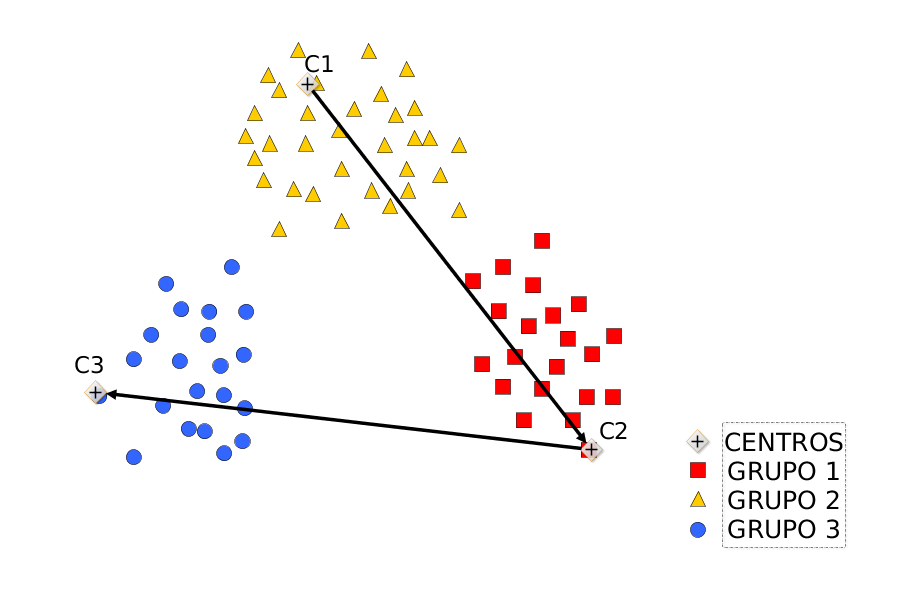
\includegraphics[width = 11cm, height = 8cm]{figuras/kmeans++.png}
\caption{\scriptsize{Distribuição dos centros inicias com Kmeans++.}}
\label{fig2}
\end{figure}

\indent Primeiramente, o algoritmo escolhe o primeiro centro de forma randômica, depois, é calculada a distância de cada ponto $x$ em relação ao centro já escolhido. E então, é escolhido como o próximo centroide o objeto que possuir a probabilidade proporcional à distância $D(x)^{2}$. Deste modo, os centros inciais são distribuídos nos pontos extremos da base de dados, impossibilitando que iniciem próximos e em um mesmo grupo.

\indent A representação da aplicação do Kmeans++ é demonstrada na figura~\ref{fig2}, no qual, o centro C1 é escolhido randomicamente, C2 é escolhido por ter a maior distância em relação ao C1 e C3 é escolhido por ter a maior distância de C2.

\indent No experimento 1 na figura~\ref{fig3}, é apresentado o funcionamento do algoritmo K-means, onde,  é realizada a clusterização em uma base contendo três tipos de tráfego: normal e os ataques do tipo \textit{smurf} e \textit{teardrop}, sendo representados respectivamente pelos grupos 1, 2 e 3. Este experimento também é utilizado como fase de treinamento, obtendo-se os seus centros finais para serem utilizados como centro iniciais em outras clusterizações.
  
\begin{figure}[!h]
\centering
\includegraphics[width = 13cm, height = 10cm]{figuras/exp1.png}
\caption{\scriptsize{Experimento 1.}}
\label{fig3}
\end{figure}

\begin{figure}[!h]
\centering
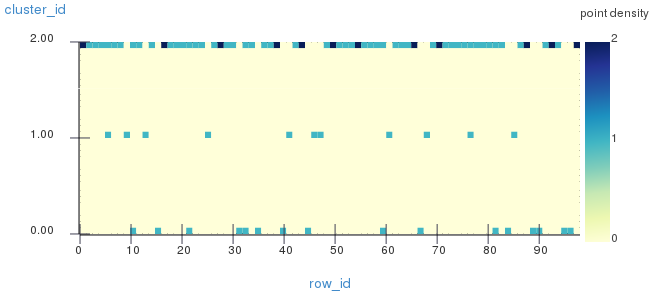
\includegraphics[width = 14cm, height = 8cm]{figuras/densidade1.png}
\caption{\scriptsize{Densidade de elementos do experimento 1.}}
\label{fig4}
\end{figure}
  
\newpage

\indent A fase de testes é representada pelo experimento 2 na figura~\ref{exp2}, onde os centros obtidos na fase de treinamento, são reutilizados como centros iniciais. Nesta fase os dados estão distribuídos randomicamente na base, diferente do que ocorre no experimento da figura~\ref{fig3}, em que os dados foram alocados ordenadamente.

\begin{figure}[!h]
\centering
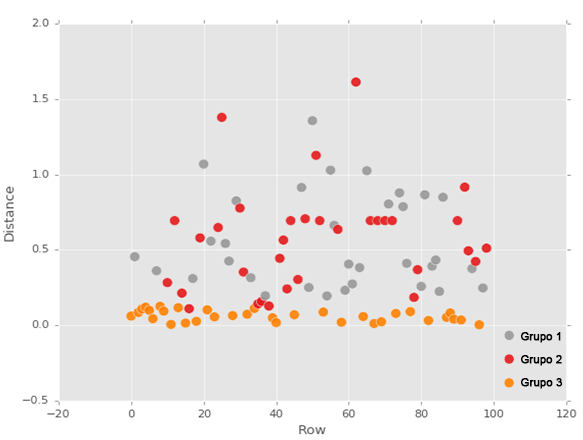
\includegraphics[width = 13cm, height = 10cm]{figuras/aleatorio1.png}
\caption{\scriptsize{Experimento 2.}}
\label{exp2}
\end{figure}

\begin{figure}[!h]
\centering
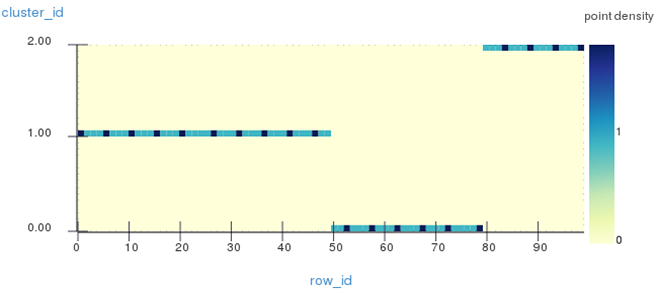
\includegraphics[width = 14cm, height = 8cm]{figuras/densidade2.png}
\caption{\scriptsize{Densidade de elementos do experimento 2.}}
\label{fig6}
\end{figure}

\indent Nota-se que a clusterização ocorre como no primeiro experimento, conseguindo classificar corretamente todos os dados, mesmo com a distribuição randômica. Porém, caso sejam utilizados ataques que compartilhem características mais semelhantes, pode ocorrer de alguns elementos serem classificados erroneamente.

\indent Pode-se analisar também a densidade e quantidade de elementos nos três grupos do experimento 1 na figura~\ref{fig4} e do experimento 2 na figura~\ref{fig6}, sendo possível visualizar a respectiva linha de cada vetor de conexão e suas intercalações na base de dados.

    \section{Resultados}

\indent Por possuirmos a correta rotulagem dos dados, é possível realizar a aplicação de métodos que avaliem o desempenho e a generalização dos modelos de treinamento utilizados para a clusterização dos dados \cite{Tan2005}.

\indent O método de \textit{Cross Validation} permite a avaliação dos modelos de treinamento utilizado para definição dos centros iniciais dos novos \textit{clusters} na fase de testes. Também permite calcular as taxas de acertos e de erros resultados da aplicação do algoritmo. O método consiste na divisão da base de dados em \textit{K} partes que possuam aproximadamente o mesmo número de elementos. O subconjunto de treinamento é constituído de \textit{K} - 1 partes e o subconjunto de testes é composto pela parcela restante dos dados. A operação deve ser realizada \textit{K} vezes, de um modo que todas as partes tenham sido utilizadas no subconjunto de testes.

\indent O conjunto de dados utilizado para os experimentos de \textit{Cross Validation} será assim como o utilizado no experimento 2, com a mesma quantidade de vetores de conexão e a distribuição randômica dos dados. Além disso, será utilizado o valor de \textit{K} = 3, onde, os subconjuntos de treinamento serão compostos por 2/3 dos dados e os subconjuntos de teste serão compostos por 1/3 do total de dados, variando em cada iteração.

\indent Na tabela~\ref{tab5}, as taxas de falsos positivos e verdadeiros positivos, são referentes à detecção de anomalias. Sendo assim, elas indicam se os ataques foram classificados nos grupos anômalos, independente de estarem no seu específico grupo de ataque. E se os dados normais foram agrupados corretamente, não estando presentes nos grupos anômalos. A taxa de falsos positivos é representada pela equação (\ref{eq:Fp}) e a taxa de verdadeiros positivos pela equação (\ref{eq:Vp}).

\vspace{0.3cm}
\begin{equation}
\label{eq:Fp} %Título da equacao
\textrm{Taxa de falso positivo} = \frac{\textrm{Quantidade de falsos positivos}}{\textrm{Quantidade de dados normais}}
\end{equation}
\vspace{0cm}

\vspace{0cm}
\begin{equation}
\label{eq:Vp} %Título da equacao
\textrm{Taxa de verdadeiro positivo}  = \frac{\textrm{Quantidade de verdadeiros positivos}}{\textrm{Quantidade de dados anômalos}}
\end{equation}
\vspace{0.3cm}

\indent As taxas de acertos e erros, respectivamente representadas pelas equações (\ref{eq:Acertos}) e (\ref{eq:Erros}), são referentes ao agrupamento em si. Deste modo, avaliam se os elementos foram classificados em seus respectivos grupos, não levando em consideração as classificações anômala ou normal. Assim, mesmo que um ataque não seja considerado normal, mas tenha sido alocado no grupo de um outro ataque, um erro será contado.

\vspace{0.3cm}
\begin{equation}
\label{eq:Acertos} %Título da equacao
\textrm{Taxa de acertos} = \frac{\textrm{Quantidade classificações corretas}}{\textrm{Número total de elementos}}
\end{equation}
\vspace{0cm}

\vspace{0.3cm}
\begin{equation}
\label{eq:Erros} %Título da equacao
\textrm{Taxa de erros} = \frac{\textrm{Quantidade classificações incorretas}}{\textrm{Número total de elementos}}
\end{equation}
\vspace{0cm}

\begin{table}[h]
\centering
\caption{\textit{Cross Validation} 1 (situação ótima).}
\vspace{0.5cm}
\begin{tabular}{|c|c|c|c|c|}
\hline
\textbf{Etapa K} & \textbf{Falso Positivo} & \textbf{Verdadeiro Positivo} & \textbf{Acertos} & \textbf{Erros}\\
\hline
1 & 0\% & 100\% & 100\% & 0\% \\
\hline
2 & 0\% & 100\% & 100\% & 0\%\\
\hline
3 & 0\% & 100\% & 100\%& 0\%\\
\hline
\end{tabular}
\label{tab5}
\end{table}

\indent As taxas apresentadas na tabela~\ref{tabela6}, são referentes à validação do experimento 2, um caso em que houve solução ótima do agrupamento. Em todas as iterações do \textit{cross validation} todos os elementos foram classificados corretamente . Isso ocorre devido à grande quantidade de atributos com valores e padrões díspares entre o tráfego normal e os ataques \textit{smurf} e \textit{teardrop}. Como, por exemplo, os protocolos de aplicação e de transporte e a quantidade de \textit{bytes} enviados, que assim como outros atributos, mantêm um valor contínuo nos ataques, enquanto são variantes no tráfego normal.

\indent Ao utilizar o tráfego normal juntamente com os ataques \textit{neptune} e \textit{back} em uma base de mesmas dimensões como foi utilizada na validação anterior, há uma situação em que os atributos de cada tipo de tráfego possuem muitas características semelhantes, propiciando uma situação em que o algoritmo consegue reconhecer alguns elementos de cada grupo, mas não possui tamanha exatidão como na validação anterior. 

\begin{table}[h]
\centering
\caption{\textit{Cross Validation} 2.}
\label{tabela6}
\vspace{0.5cm}
\begin{tabular}{|c|c|c|c|c|}
\hline
\textbf{Etapa K} & \textbf{Falso Positivo} & \textbf{Verdadeiro Positivo} & \textbf{Acertos} & \textbf{Erros}\\
\hline
1 & 81,82\% & 100\% & 45,45\% & 54,55\% \\
\hline
2 & 33,33\% & 91,67\% & 60,61\% & 39,39\%\\
\hline
3 & 0\% & 100\% & 57,58\% & 42,42\%\\
\hline
\end{tabular}
\end{table}

\indent Os dados da desta validação são apresentados na tabela~\ref{tabela6}, e pode-se verificar que o modelo de treinamento com melhor desempenho foi o de \textit{K} = 2, em que os dados de treinamento foram retirados da parte superior e inferior da base de dados, enquanto os dados de teste foram retirados do centro da base.

\indent Para aproximar os experimentos a um ambiente real, na seguinte validação foram utilizados os mesmos tipos de tráfegos do experimento anterior, porém, as dimensões da base foram aumentadas  para cerca de vinte e dois mil vetores de conexão, onde 60\% são de dados normais e o restante é composto pelos ataques. Estas dimensões foram escolhidas baseando-se na premissa de que há uma maior quantidade de dados normais do que anômalos em um tráfego real.

\begin{table}[h]
\centering
\caption{\textit{Cross Validation} 3.}
\label{tabela7}
\vspace{0.5cm}
\begin{tabular}{|c|c|c|c|c|}
\hline
\textbf{Etapa K} & \textbf{Falso Positivo} & \textbf{Verdadeiro Positivo} & \textbf{Acertos} & \textbf{Erros}\\
\hline
1 & 2,67\% & 0,35\% & 59,62\% & 40,37\% \\
\hline
2 & 2,93\% & 43,17\% & 75,63\% & 24,37\%\\
\hline
3 & 2,68\% & 42,56\% & 75,26\% & 27,72\%\\
\hline
\end{tabular}
\end{table}

\indent Apesar da utilização dos mesmos tipos de tráfego da validação da tabela~\ref{tabela6}, nota-se grande diferença nos resultados apresentados na tabela~\ref{tabela7}. Devido à maior quantidade de elementos normais, há uma boa diminuição nas taxas de falsos positivos em relação à validação anterior. Porém, o algoritmo também detecta uma menor quantidade de verdadeiros positivos. Além disso, nesta validação, a primeira etapa obteve um desempenho muito inferior em relação às outras duas etapa, que apresentaram resultados aproximados.

\indent Estes experimentos indicam que o algoritmo foi capaz de classificar acima de 59\% dos elementos do tráfego em seus grupos corretamente, tanto com uma base de dimensões menores, quanto com uma base semelhante à uma série temporal de tráfego real. Os experimentos da tabela~\ref{tabela6} e da tabela~\ref{tabela7} envolvem uma situação onde as características do tráfego normal são muito semelhante ao tráfego anômalo. Além disto, o tráfego anômalo é composto por dois tipos de ataques de negação de serviço muito similares, o que propiciou uma situação desvantajosa para o algoritmo e causou um menor desempenho do agrupamento.





